\documentclass{article}
\usepackage[utf8]{inputenc}
\usepackage{amsmath}
\usepackage{amssymb}
\usepackage{listings}
\usepackage{graphicx}
\usepackage{wrapfig}

\begin{document}

\section*{Computing a Level Set}
We define for a real-valued function $f : D \subset \mathbb{R}^{d} \to \mathbb{R}$ the level sets by the following definition.
\begin{equation*}
    \mathcal{L}_{c}:= \left\{\mathbf{x}\in D \: : \: f\left(\mathbf{x}\right) \leq c\right\} \: \text{,} \quad c \in \mathbb{R}
\end{equation*}
Let $f : \mathbb{R}^{2} \to \mathbb{R}$ be a continuously differentiable \textbf{strictly convex} function which has a \textbf{global minimum} in $\mathbf{x} = 0$ and satisfies the growth condition $\left\lvert f\left(\mathbf{x}\right) \right\rvert \to \infty$ uniformly for $\left\lVert \mathbf{x}\right\rVert \to \infty$.  The level sets $\mathcal{L}_{c}$ for $D = \mathbb{R}^{2}$ and $c > 0$ will be closed and convec subsets of $\mathbb{R}^{2}$ Every ray
\begin{equation*}
    R_{\mathbf{d}} := \left\{\,\xi\mathbf{d} \: : \: \xi \geq 0\,\right\}\,\text{,} \quad \mathbf{d} \in \mathbb{R}^{2} \setminus \left\{\mathbf{0}\right\}
\end{equation*}
will intersect the boundary of $\mathcal{L}_{c}$
\begin{equation*}
    \partial \mathcal{L}_{c} := \left\{\mathbf{x} \in \mathbb{R}^{2} \: : \: f\left(x\right) = c\right\}
\end{equation*}
\paragraph{8-13.a} We are tasked with stating a Newton iteration for the intersection between the ray $R_{\mathbf{d}}$ and the boundary of $\mathcal{L}_{c}$ given by $\partial\mathcal{L}_{c}$. We are given point evaluations of $f$ and $\text{\textbf{grad}}\, f$. We want to solve
\begin{equation*}
    \xi \mathbf{d} = x \: \land \: f\left(x\right) = c \implies f\left(\xi \mathbf{d}\right) = c
\end{equation*}
Because we are interested in solving this using a Newton iteration we will have to transform this into a root finding problem
\begin{equation*}
    f\left(\xi \mathbf{d}\right) - c = 0
\end{equation*}
We have
\begin{equation*}
    F\left(\xi\right) = f\left(\xi \mathbf{d}\right) - c = 0
\end{equation*}
and
\begin{equation*}
    F'\left(\xi\right) = \text{\textbf{grad}}\, f\left(\xi\mathbf{d}\right)^{\mathsf{T}} \cdot \left(\xi \mathbf{d}\right)' = \text{\textbf{grad}}\, f\left(\xi\mathbf{d}\right)^{\mathsf{T}} \cdot \mathbf{d}
\end{equation*}
We hence get (the data points are dependent on $\xi$)
\begin{equation*}
    \xi^{\left(k+1\right)} = \xi^{\left(k\right)} - \frac{F\left(\xi^{\left(k\right)}\right)}{F'\left(\xi^{\left(k\right)}\right)} = \xi^{\left(k\right)} - \frac{f\left(\xi^{\left(k\right)}\mathbf{d}\right)-c}{\text{\textbf{grad}}\, f\left(\xi^{\left(k\right)}\mathbf{d}\right)^{\mathsf{T}}\mathbf{d}}
\end{equation*}
Because $\xi \geq 0$ per definition of the set $R_{\mathbf{d}}$ we need to choose $\xi^{\left(0\right)} > 0$. As always with the Newton's method we need to assure that the denominator cannot vanish, we have that $\mathbf{d} \in \mathbb{R}^{2} \setminus \left\{\mathbf{0}\right\}$, also we have that $f$ is strictly convex and hence $\text{\textbf{grad}}\, f\left(\xi^{\left(k\right)}\mathbf{d}\right)$ is strictly increasing and since the global minimum is at $\mathbf{x} = 0$ it must be non-zero for any other value $\mathbf{x} > 0$. Hence the denominator can never be zero and the Newton iteration is well-defined. 
\subsection*{8-13.b} We now want to do the same thing for the \textbf{secant method} we have seen the secant line is given by 
\begin{equation*}
    s\left(\xi\right) = F\left(\xi^{\left(k\right)}\right) + \frac{F\left(\xi^{\left(k\right)}\right) - F\left(\xi^{\left(k-1\right)}\right)}{\xi^{\left(k\right)}-\xi^{\left(k-1\right)}}\left(\xi - \xi^{\left(k\right)}\right)
\end{equation*}
From this we get the secant iteration
\begin{equation*}
    \xi^{\left(k+1\right)} = 
 \xi^{\left(k\right)} -\frac{F\left(\xi^{\left(k\right)}\right)\left(x^{\left(k\right)} - \xi^{\left(k-1\right)}\right)}{F\left(\xi^{\left(k\right)}\right)-F\left(\xi^{\left(k-1\right)}\right)}
\end{equation*}
We need two initial guesses, so we choose $\xi^{\left(0\right)}$ such that $F\left(\xi^{\left(0\right)}\right) <0$ and $\xi^{\left(1\right)}$ such that $F\left(\xi^{\left(1\right)}\right) >0$. Written using the definition of $F$ we get
\begin{equation*}
   x^{\left(k+1\right)} = x^{\left(k\right)} -\frac{\left(f\left(\xi^{\left(k\right)}\mathbf{d}\right)-c\right)\left(\xi^{\left(k\right)} - \xi^{\left(k-1\right)}\right)}{f\left(\xi^{\left(k\right)}\mathbf{d}\right) - c -f\left(\xi^{\left(k-1\right)}\mathbf{d}\right)+c} = \xi^{\left(k\right)} -\frac{\left(f\left(\xi^{\left(k\right)}\mathbf{d}\right)-c\right)\left(\xi^{\left(k\right)} - \xi^{\left(k-1\right)}\right)}{f\left(\xi^{\left(k\right)}\mathbf{d}\right)  -f\left(\xi^{\left(k-1\right)}\mathbf{d}\right)}
\end{equation*}

\subsection*{8-13.c}
We are given the following method to implement
\begin{lstlisting}[language=C++,
                   directivestyle={\color{black}}
                   emph={int,char,double,float,unsigned},
                   emphstyle={\color{blue}}
                  ]
template <typename Functor>
Eigen::Vector2d pointLevelSet(Functor&& f, 
                              const Eigen::Vector2d& d, double c,
                              const Eigen::Vector2d& x0, 
                              double rtol = 1e-10,
                              double atol = 1e-16) {


}
\end{lstlisting}

We can see that we are given the function $f$, the vector $d$, the value $c$, both \textit{relative} and \textit{absolute} tolerance and the point $x_{0}$. We are then tasked to choose two suitable initial points. The task description presents the following two points
\begin{equation*}
    p_{1} = \frac{\left\lVert x_{0}\right\rVert_{2}}{\left\lVert d\right\rVert_{2}}\mathbf{d}  \qquad p_{2} = 1.1 \cdot \frac{\left\lVert x_{0}\right\rVert_{2}}{\left\lVert d\right\rVert_{2}}\mathbf{d}
\end{equation*}
As the secant as shown in the script on page 616 works only for initial points with a real value we will choose the following initial points
\begin{equation*}
    a = \frac{\left\lVert x_{0}\right\rVert_{2}}{\left\lVert d\right\rVert_{2}}  \qquad b = 1.1 \cdot \frac{\left\lVert x_{0}\right\rVert_{2}}{\left\lVert d\right\rVert_{2}}
\end{equation*}
and then use a suitable functor that always multiplies the initial points by $\mathbf{d}$.

\pagebreak

\noindent The code given in the lecture document looks as follows.

\begin{figure}[!hbt]
    \centering
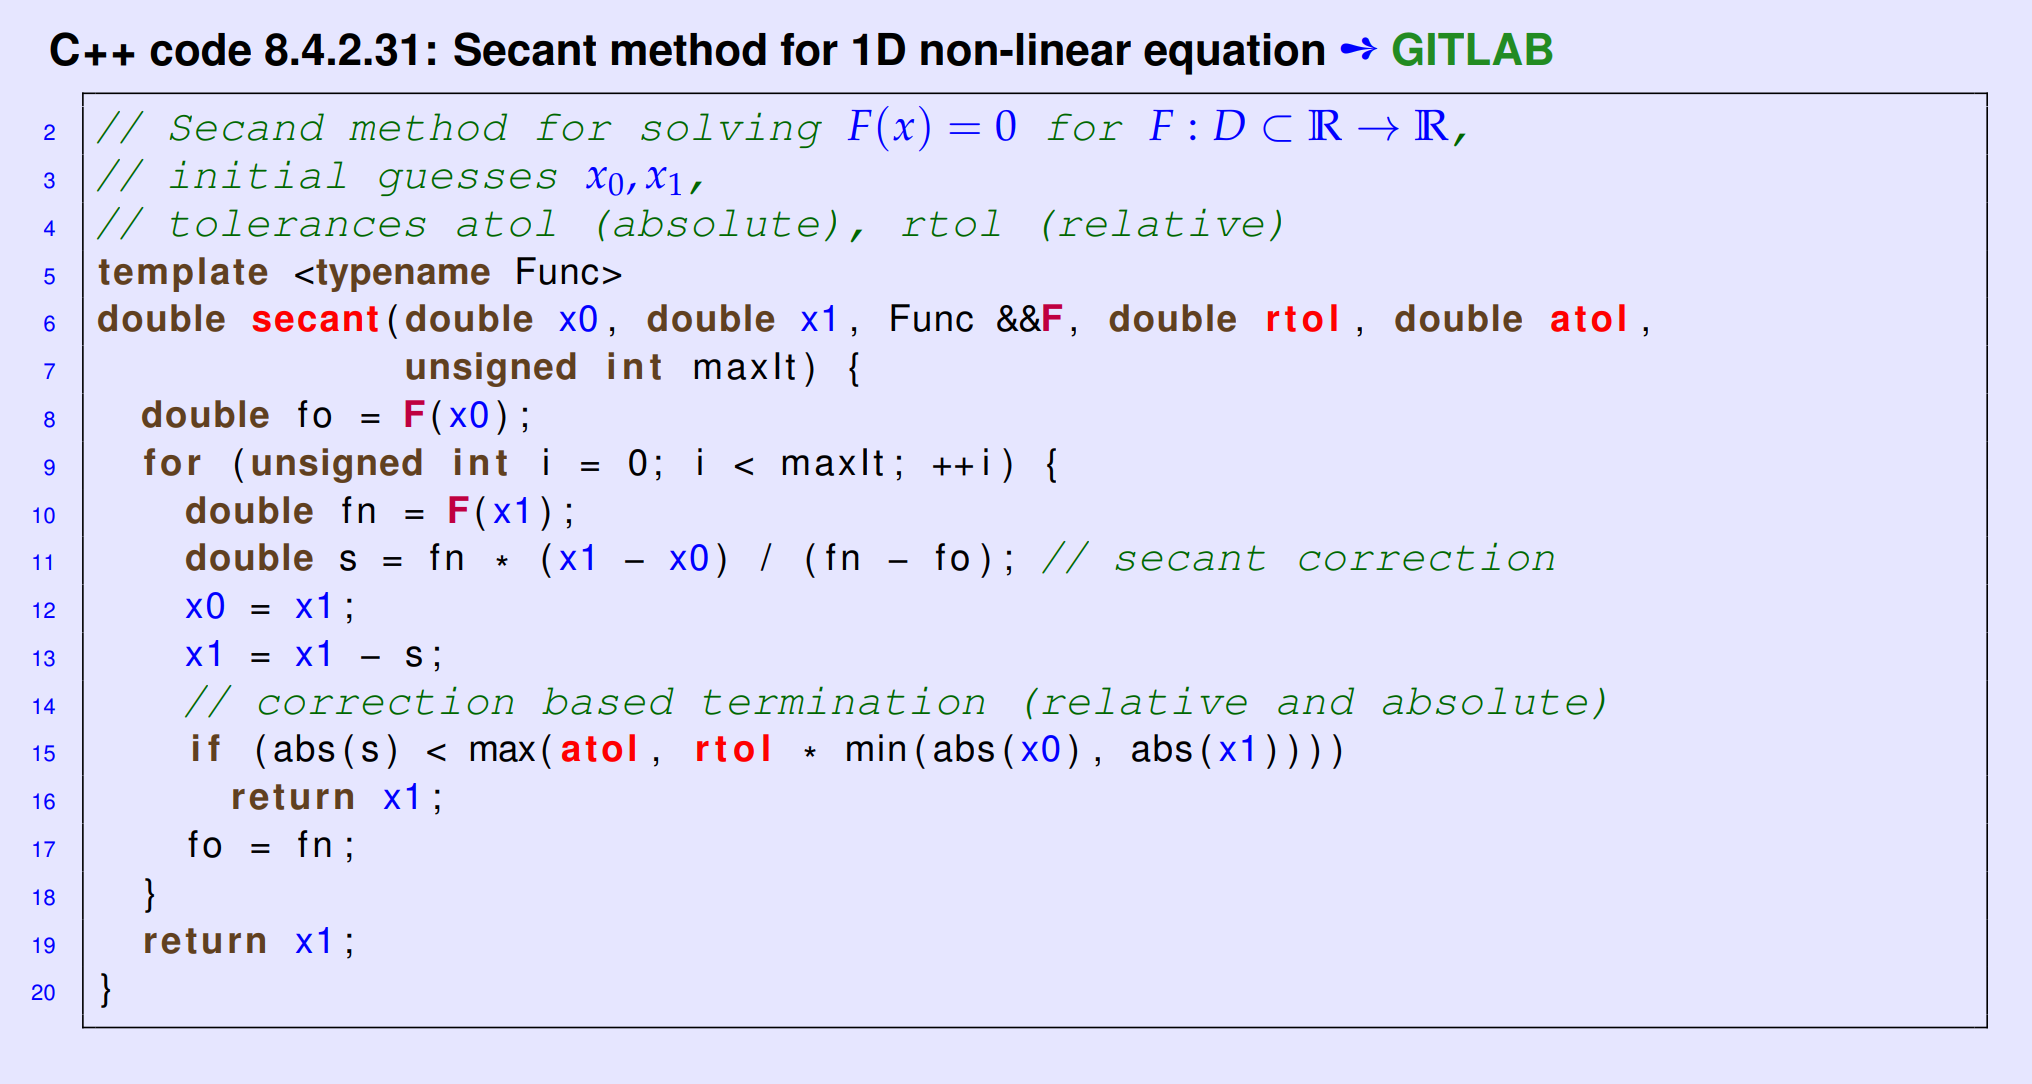
\includegraphics[width=1.0\linewidth]{SecantMethodCode.png}
\end{figure}

\noindent We can hence work very similarly, however we cannot directly use $f$ as we operate with $F$ in the secant method, as we saw in (8-13.b). The function $F$ is given to us by 
\begin{equation*}
    F\left(x\right) = f\left(x\mathbf{d}\right) - c
\end{equation*}
We can represent this in a C++ functor, the generic structure of a lambda expression looks like
\begin{equation*}
    \underbrace{\left[\,e_{1}, \dots, e_{n}\,\right]}_{\substack{\text{captures} \\ \text{(potentially none)}}} \: \: \underbrace{\left(\,T_{1} \, x_{1}\,,\dots\,, T_{m}\, x_{m}\,\right)}_{\substack{\text{parameters} \\ \text{(potentially none)}}} \: \: \: \underbrace{\:\rightarrow \: \: \text{R }}_{\text{return type}} \: \: \underbrace{\left\{ \: \text{statements} \: \right\}}_{\text{body}}
\end{equation*}
We must capture (by reference) $f$, $\mathbf{d}$ and $c$. We will accept one parameter which will be $a$ or $b$ in our case, we will return a value of type \textbf{double} and the body will contain the computation of the function value defined above. If it is unclear why lambdas capture any variables at all the have a look at this answer on StackOverflow given by \textit{newacct}: $\\[1mm]$
\noindent
"Lambdas can use variables from an outer scope. However, if those are local variables, they \textbf{go out of scope} and cannot be used after the function returns. But a lambda could potentially be called after the function returns (the lambda could be returned from the function, or stored in some global or instance variable, etc.), and after the function returns, \textbf{it cannot just refer to the local variables directly, because they no longer exist.}" $\\[1mm]$
We hence get the following lambda expression for the functor $F$

\begin{lstlisting}[language=C++,
                   directivestyle={\color{black}}
                   emph={int,char,double,float,unsigned},
                   emphstyle={\color{blue}}
                  ]
auto F = [&f, &d, &c](double t) -> double { return f(t * d) - c; };
\end{lstlisting}

\pagebreak

\noindent Now we basically just copy \& paste the code given in the lecture document , where the definition of the functor is left out, but would have to be added as well.

\begin{lstlisting}[language=C++,
                   directivestyle={\color{black}}
                   emph={int,char,double,float,unsigned},
                   emphstyle={\color{blue}}
                  ]
double a = x0.norm() / d.norm();
double b = 1.1 * a;

double s = 1.0;
double f0 = F(a);

while(std::abs(s) > std::max(atol, rtol * std::min(a, b))) {
    double fn = F(b);

    s = fn * (b - a) / (fn - f0);

    a = b;
    b = b - s;
    f0 = fn;
}

intersect = b * d;
\end{lstlisting}

We have to keep in mind that the result is not a double but of the form $x \mathbf{d}$ and hence this is why we have to set \textit{intersect} to $b \cdot \mathbf{d}$.
\subsection*{8-13.d} We have seen that we can use both the Newton's and the secant method to find intersects between a convex set and a ray. We now have a working implementation of the secant method that does this. $\\[1mm]$
\noindent The first hint tells us that a convec polygonal domain $P$ with $\mathbf{0} \in P$ can be partitioned into (non-overlapping) triangles with one vertex in $\mathbf{0}$ and the other two vertices coinciding with corners of $P$. We will hence approximate the are enclosed by a convex level set boundary (which we can do using the intersect finding technique discussed in earlier exercises) by the sum of areas of triangles having the same angle $\frac{2\pi}{n}$ at vertex 0. The area of a triangle $\Delta \, ABC$ with angle $\alpha$ at vertex $A$ is 
\begin{equation*}
    \left\lvert \Delta \, ABC\right\rvert = \frac{1}{2}\cdot \overline{AB} \cdot \overline{AC}\cdot \sin\left(\alpha\right)
\end{equation*}
We want to use the function $\textbf{pointLevelSet}$, hence let us find which are the parameters. Immediately we can see that $\mathbf{d}_{j}$ will be $\mathbf{d}$, $c$ is already given to us directly, $f$ we can pass as is, $x_{0}$ must be chosen initially. We can see that rtol and atol have a default initialization, hence no need to do anything with them. Hence we find all points were the ray given by $\mathbf{d}_{j}$ intersects with the level set given by $c$ and we store them in a vector. As an initial guess we choose $x_{0} = \left(1, 0\right)$ The area will then be given by the product of adjacent radii summed up. This works because as we compute the intersect we will directly get the length of the line between each of the triangles when taking the norm and hence the length of the corresponding side. We can thus just multiply the adjacent sides and call it a day after summing these sub-results up. 

\subsection*{8-13.e} 
We are given the following table of error data.

\begin{figure}[!hbt]
    \centering
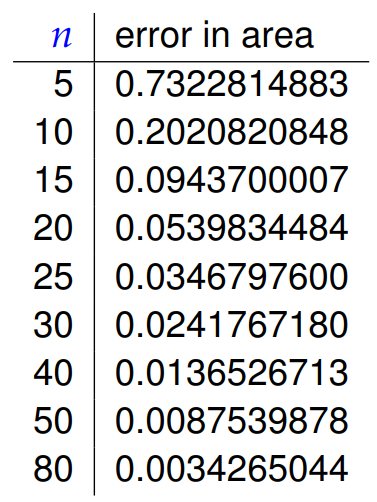
\includegraphics[width=0.3\linewidth]{ErrorData.png}
\end{figure}

for the function
\begin{equation*}
    f\left(\mathbf{x}\right) = x_{1}^{2} + 2x_{2}^{4} \, \text{,} \quad \mathbf{x} = \begin{bmatrix}
        x_{1} \\ x_{2}
    \end{bmatrix} \in \mathbb{R}^{2}
\end{equation*}
We use this function and compute the area using the \textbf{areaLevelSet} method. We look at the error data and see that between $5$ and $10$ we get a decrease of the error of $0.73222 / 0.20208 \approx 3.6$, between $10$ and $20$ we get $0.20208 / 0.05398 \approx 3.8$ , between $20$ and $40$ we get $0.05398 / 0.01365 \approx 4$ and between $40$ and $80$ we get $0.01365 / 0.0034265 \approx 4$. We hence approximately reduce the error by a factor of $4$ while increasing $n$ by a factor of $2$. While $n$ will grow the error decreases and we have a algebraic convergence with rate $2$, we have a linear growth for $n$ and a $n^{-1}$ growth for the error, while the error decreases faster than $n$ by a square relationship ($4 = 2^{2}$) and we hence get
\begin{equation*}
    \text{error} = \mathcal{O}\left(\left(\frac{1}{n}\right)^{2}\right) \quad \text{for } n \to \infty 
\end{equation*}

\end{document}
